\documentclass[]{report}
\title{Wireless Modular Diagnostic Tooling}
\author{Douglas Palmer \and Joseph Lenox \and Nick Hamann \and Matthew Morgan \and Wesley Trendinnick}
\date{April 21, 2008}

\usepackage{fancyhdr}
\usepackage{makeidx}
\usepackage{multirow}
\usepackage{pdfpages}
\usepackage{listings}
\usepackage{color}
\usepackage{cite}
\usepackage{url}
\usepackage[pdftitle={Report: Wireless Modular Diagnostic Tooling},colorlinks=false]{hyperref}
\pagestyle{fancy}
\makeindex
% start the document
\begin{document}
\maketitle
\tableofcontents

\stepcounter{section}
\addcontentsline{toc}{section}{\numberline{\roman{section}}Acknowledgements}
\section*{Acknowledgements}
\begin{itemize}
\item Dr. Haibo Wang, for his assistance during reviews of the design. 
\item Dr. Spyros Tragoudas, for his advice during the review of the design.
\item Gladys Hounsinou provided prototyping boards and logic chips.
\item Nancy Beasley provided computer hardware for use.
\end{itemize}

\paragraph{Credits}
\begin{itemize}
\item Joseph Lenox
\item Wesley Trendinnick
\item Nick Hamann
\item Douglas Palmer
\item Matthew Morgan
\end{itemize}

\chapter{Subsystem Discussions}
%include subsystem reports here.
%like this: \include{report_name}
%report_name is the name of the .tex file, without the extension.
% Subsystem Report for the Analog Input Module system.
\fancyfoot[R]{WT}
\section[Analog Input]{Analog Input Module Subsystem}
\subsection{Description}
The purpose of the signal conditioning subsystem is to scale the analogue input
 to an appropriate level so that it can be read by the analogue to digital 
converter. The goal is to scale the output voltage to be between 0 and 5 volts 
and allow proper shifting and amplification via user interaction with the 
software. 

As per Figure \ref{fig:analog drawing}, this was implemented using 4 operational amplifiers, a digital to analogue converter, a multiplexer, resistors, and diodes. 741 operational amplifiers were chosen for this circuit because they are the most inexpensive op amps to purchase and their specs allow for them to be used in this circuit. A reference voltage of +/- 12 volts was used to supply these op amps, which allow for a maximum of +/- 22 volts\cite{ds:741 op amp}.

The input voltage is allowed to range from -12.7 volts to +12.7 volts. The 
diode and resistor configuration shown in drawing 201 assures the input voltage cannot vary outside of this range. These standard diodes and resistors were chosen because only basic diodes and resistors were needed and these components were very inexpensive. This input voltage is applied to the non-inverting input of an operational amplifier. The output of this op amp goes back to the inverting op amp, so it acts as a voltage follower\cite{bk:olia}.

Another voltage is produced from a digital to analogue converter. This voltage
 ranges from 0 to 5 volts. The purpose of the digital to analogue converter is
 to shift the signal up and down. The user controls this shift using the
 software on the computer. Because this requires communication with the micro
 controller, a digital to analogue converter was chosen with an 
I$^2$C interface. Consequently the PCF8591 was selected to 
produce a voltage ranging from 0 to 5 that goes into the non-inverting input 
of an op amp. This op amp also acts as a voltage follower.

These 2 voltages were each placed in series with a 10k resistor and both 
connected to the inverting input of another op amp. This op amp serves to 
amplify the voltage signal. Essentially the output from this op amp is the sum
 of the input and DAC voltages multiplied by the amplification[5]. The 4067
 analogue multiplexer is used to select the appropriate resistance. Like the 
digital to analogue converter, the multiplexer gets information from the micro
 controller and activates the desired output to use a resistor. These
 resistors vary from 10k ohms to 1M ohms to allow for different levels of 
amplifications. For example, for 2x amplification, the 20k resistor is used 
($20k/10k = 2x$ amplification) and this is multiplied by the sum of the 
earlier voltages\cite{bk:olia}.

The final op amp is used to scale the signal down to between 0 and 5 volts for 
the analogue to digital controller to read. An inverting op amp configuration 
is used with 3 volts going into the non-inverting input.
The output of this op amp is then sent to the analogue to digital converter.
Figure 201 and table 201 summarize the different parts of the circuit.

\subsection{Implementation}
Constructing the circuit is straight-forward and the connections can be seen 
from Figure \ref{sch:signal amp}. Setting up the circuit to be tested requires 
multiple voltage sources. Setting up the source voltages can be a little tricky.
Since the 741 op amps are not rail to rail, the +12 and -12 reference voltages 
must be supplied using 2 different voltage sources[1]. 

If the circuit is going to be implemented separately from the micro controller, another voltage source should be used as the voltage to the op amp by circle 
2 in figure 201. Another voltage source of 3 volts should be applied to the 
non-inverting input of the op amp by circle 6 in figure 201. Finally the input 
voltage should be applied to circle 1 in figure 201. Finding multiple power 
supplies is necessary before testing the unit as a whole. 
The feedback resistor of the op amp by circle 5 in figure 201 can be manually 
placed there instead of through the multiplexer if being tested without the 
micro controller. 

To start off, the voltage clamp of the diodes and resistors by circle 1 in 
figure 201 is tested. Use a multimeter to test the voltage before it reaches 
the first op amp. Adjust the input to points outside the + and -12.7 volts. 
The output should not be bellow -12.7 nor above +12.7 volts[1]. 
	Next, test the op amps by circles 2 and 3 in figure 201 and make sure the 
output voltage is equal to the input. Then record the voltage coming out of the
 op amp by circle 5 in figure 201 with 10k feedback. This should be 
approximately equal to the inversion of the sum of the input and digital to 
analogue voltages\cite{bk:olia}.
The feedback resistor of the op amp by (5) in Figure figure 201 can be manually
 placed there instead of through the multiplexer if being tested without the 
micro controller. 

The voltage clamp of the diodes and resistors by (1) in
 Figure\ref{sch:signal amp} should be tested first. Use a multimeter to test
 the voltage before it reaches the first op amp. Adjust the input to points 
outside the + and -12.7 volts. The output should not be below -12.7, nor 
should it be above +12.7 volts.

Next, test the op amps by circles 2 and 3 in figure 201 and make sure the 
output voltage is equal to the input. Then record the voltage coming out of 
the op amp by circle 5 in figure 201 with 10k feedback. This should be 
approximately equal to the inversion of the sum of the input and digital to 
analogue voltages\cite{bk:olia}. \begin{equation} V = -[V_{DAC} + V_{IN}]\end{equation}

If this is correct, finally test the output voltage coming out of the op amp by
 circle 6 in . Put the input voltage to the max of 12.7 and the DAC 
voltage to its max of 5. This should yield an output of 0. Then set the input 
voltage to -12.7 and the DAC voltage to 0. The output voltage should be around 
5 volts. Any other input voltage levels should show an output voltage between 0 and 5 and be approximately:

\begin{equation}\label{vout}V_{OUT} = 3 - .16447[V_{DAC} + V_{IN}]\end{equation}

When testing the circuit, the actual output voltage did not match up with the 
theoretical output described by \eqref{vout}. Table \ref{tbl:analog input data}
 shows the different input voltages and the resulting outputs of the
 theoretical and actual voltages.

Although these results did not match up precisely with what was expected, they 
are still within the range of the analogue to digital converter to read. They 
were just scaled to different values.

\subsection{Fault Analysis}
There are several obvious but overlooked reasons as to why this circuit 
would not operate properly. Understanding the op amp is key to knowing what is
 wrong. During preliminary testing, the op amp was not showing any output
 voltage when constructed as a voltage follower. After many attempts, no output
 voltage could be obtained. Finally the op amp was moved to another part of
 the breadboard and it operated correctly right away. A part of the breadboard
 used was not operating correctly. A faulty breadboard can be tested with a 
multimeter to make sure the connections are properly working.

It is possible to ruin the diodes or op amps if excess voltage is give to
 them. If the diodes are facing the wrong direction they will also not operate
 properly. If there as any doubt of the components not working correctly, get
 new parts to replace them. The diodes and op amps are cheap so it would not 
cost very much to use another one.

If the actual voltages and theoretical voltages are varying, it could be 
because of variances in each device. Make sure to use resistors with gold (5\%)
 tolerances. Also, the exact measurements should be obtained before plugging
 them into the equations used, not the theoretical values.
	It is recommended to change the parameters surrounding the final op amp to 
alter the output. Changing the resistances of the negative feedback and the
 voltage level of the non-inverting output should be done to alter the output.

\subsection{Cost}
20 components must be obtained to build this circuit. Each part is shown in 
drawing 201 and table 203. 12 resistors are used. 3 1k resistors are used,
 with 2 for the voltage clamp and 1 for the final op amp. 1 6.2k resistor is
 used for the final op amp. 3 10k resistors are used with 2 being placed after
 each voltage follower and the other in the variable resistance feedback. The 
remaining 5 are used in the variable resistance feedback with values of 20k,
 50k, 100k, 500k, and 1M ohms.
	2 1N4001 diodes, 4 741 op amps, 1 4067 multiplexer, and 1 digital to
 analogue converter are also used.

\begin{figure}[hbp]
\caption{Photograph of implemented signal conditioner on breadboard}
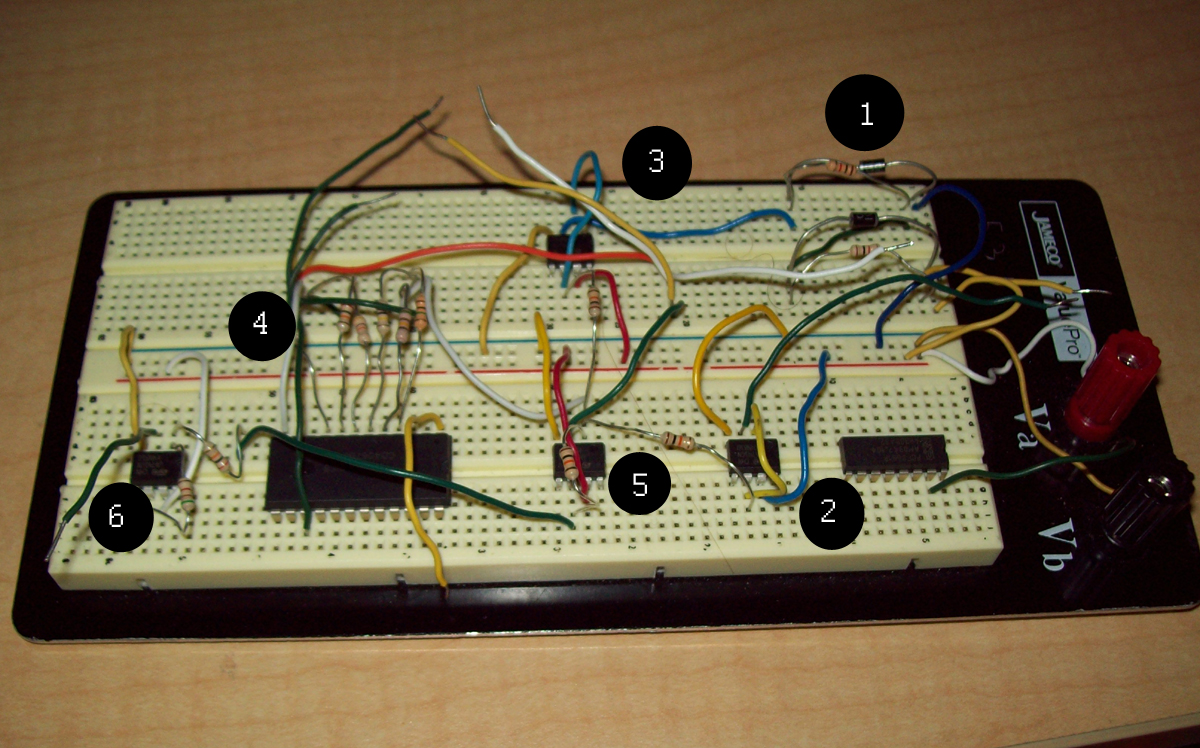
\includegraphics[width=5in]{sub_analog_hw.jpg}
\label{fig:analog breadboard}
\end{figure}

\subsection{Performance Data}
\begin{table}[hbp]
\caption[Test Results]{Expected and Actual Results (With 1x amplification)}
\begin{center}
\begin{tabular}{c| r @{.} l r @{.} l r @{.} l}  
	Input Voltage & \multicolumn{2}{r}{DAC Voltage} &
	\multicolumn{2}{r}{Theoretical Voltage} &
	\multicolumn{2}{r}{Actual Voltage} \\ \hline
	12 & 7 & 5 & 0 & 09 & 1 & 4 \\ \hline
	10 & 0 & 3 & 0 & 86 & 1 & 9 \\ \hline
	2  & 0 & 4 & 2 & 01 & 3 & 2 \\ \hline
	-12 & 7 & 0 & 5 & 08 &5 & 1 \\
\end{tabular}
\end{center}
\label{tab:analog input data}
\end{table}



% Subsystem report for Datapath control system, typeset for the LaTeX processor.
% Copy the next line and put your initials instead of JL.
\fancyfoot[R]{JL}
\section[Datapath Control]{Acquisition Unit Datapath Control}
% Description of function or purpose
\subsection{Description}
For the data acquisition hardware, a flexible base was needed to manage the 
flow of data from the analog or digital input modules to the host PC. It was 
also desired to allow the host PC to manage the configuration of the input 
modules themselves. The datapath control subsystem regulates the flow of data 
from the input modules\index{input modules} and serializes it for output to 
the host PC software. It provides a multiplexed bus for analog and/or 
digital interface modules and also provides a control interface for those 
modules. The bus width was set at 10 bits, which was the minimum size for
 accepting output from the analog input module designed for use with this 
datapath.
\subsection[Tradeoffs]{Design Decisions and Tradeoffs} 
Table \ref{tab:control comparison} lists an overview of the options considered
 for the datapath control subsystem. Cost refers to the per-unit cost of a 
given solution, Complexity is the amount of up-front design work that would
 need to be done to achieve basic functionality. TTL Logic and FPGAs are, for
 these considerations, similar. Both require much work to achieve some basic
 functionality but had very few limits in the the types of solutions that
 could be realized. FPGAs have an additional advantage over basic logic gates
 in that they are able to be relatively easily reconfigured or updating, which
 would make prottotyping simpler. However, both solutions low-level
 implementations were considered to be too time-inefficient for this design.
 A general purpose "bare" microprocessor was also considered, but was quickly
 dismissed for similar reasons as FPGAs - the infrastructure required to get
 a general microprocessor functioning was also considered time-inefficient.

\begin{table}[bp]
\caption[Controllers]{Comparison of different control methods}
\begin{tabular}{l| c c c c c c}
		\multirow{2}{*}{\small{Control Type}} & \multirow{2}{*}{\small{Cost}} 
		& \multirow{2}{*}{\small{Complexity}} & \multirow{2}{*}{\small{Flexibility}} 
		& \multirow{2}{*}{\small{Speed}} 
		& \small{Time}\\
		&&&&&\small{Required}\\ \hline
		\small{Basic logic}  &     &      &      &     & \\
		  \small{gate chips} & \small{Low} & \small{High} & \small{High} & \small{Low} & \small{V. High} \\ 
		\small{FPGA} & \small{Average} & \small{High} & \small{High} & \small{Average} & \small{High}  \\
		\small{Microprocessor} &\small{ Average} & \small{High} & \small{Average} & \small{Average}
		 & \small{Average} \\
		\small{Microcontroller} & \small{Low} & \small{Low} & \small{Average} & \small{Average} & \small{Low} \\
\end{tabular}
\label{tab:control comparison}
\end{table}

Microcontrollers, however, are ideal for this type of application: they provide
 a flexible base and generally come packaged with different interfacing 
subsystems of their own for a low cost. In addition, many microcontrollers 
have a C compiler ported for their architecture, as well as the ability to
 reprogram them in-system. Table \ref{tab:MCU capabilities} outlines some of
 the capabilties of two microcontrollers that had been under consideration.
 While the the two devices are very similar, the Atmel MCU was chosen for its
 more flexible layout, multiple integrated interfaces, and the availability
 of a mature port of the GNU C Compiler for the device (and its family). The 
PIC required the use of the vendor-supplied compiler and IDE.
\begin{table}[bhp]
\caption[Atmel and PIC MCUs]{Comparison of Atmel ATMega8515 and PIC18F1220}
\begin{tabular}{l| c c c c c c}
\setlength{\tabcolsep}{1pt}
	       &      & \small{Pin}  & \small{Maximum} & \small{Ease}   &            &         \\
	\small{Device} & \small{Cost} & \small{Count} & \small{Speed}  & \small{of Use} 
	& \small{Interfaces} & \small{Features}\\\hline
	\multirow{3}{*}{\small{ATMega8515}} & \multirow{3}{*}{\small{Low}} & \multirow{3}{*}{\small{40}}
	& \multirow{3}{*}{\small{20Mhz}} & \small{High} 
	& \small{SPI,} & \small{Timers}\\
	           &     &    &       &      &\small{USART} & \small{External}\\
	& & & & & &\small{Memory}\\\hline
	\small{PIC18F1220} & \small{Low} & \small{18} & \small{40Mhz} & \small{Average} & 
	\small{USART} & \small{Timers} \\
	           &     &    &       &      &  & \small{10-bit ADC}\\
\end{tabular}
\label{tab:MCU capabilities}
\end{table}

The bus interface features two input ports and one output port. To effectively
 switch between the two inputs, those connections must be tri-stated. Three 
74-series tri-state buffers were considered: the 74*244, the 74*245, and the 
74*621. Table \ref{tab:buffer comparison} outlines the key differences with 
the components considered. Ultimately, a 74*245 chip was selected for its 
flexibility and that there was a supply already on-site. 74*621s were found 
to be difficult to source in low quantites for a prototype. 74*244s could be 
used as well with some minor changes in glue logic, as well as 74*621s.

\begin{table}[bhp]
\caption[Buffer Comparison]{Comparison of different tri-state buffers}
\small
\begin{center}
\begin{tabular}{l| c c c c}
\setlength{\tabcolsep}{1pt}
	Device & Width & Bi-Directional & Cost & Availability \\\hline
	74*244 & 8     & No             & Low  & High\\
	74*245 & 8     & Yes            & Low  & High\\
	74*621 & 8     & Yes            & Low  & Low
\end{tabular}
\end{center}
\label{tab:buffer comparison}
\end{table}

\cite{ds:ATMEGA8515}


% The beginning of the appendix.
\fancyfoot[R]{}
\begin{appendix}
% Documents that are part of the appendix need to go here.

% All datasheets for our project.
% commented out for now. Uncomment when done
%\chapter{Datasheets}
% Analog MUX used in signal conditioner

\includepdf[pages=2-8]{../ref/CD4067.pdf}

%WT32

\includepdf[pages=-]{../ref/WT32_Datasheet.pdf}
% 74LS gates, 244 is unused.
%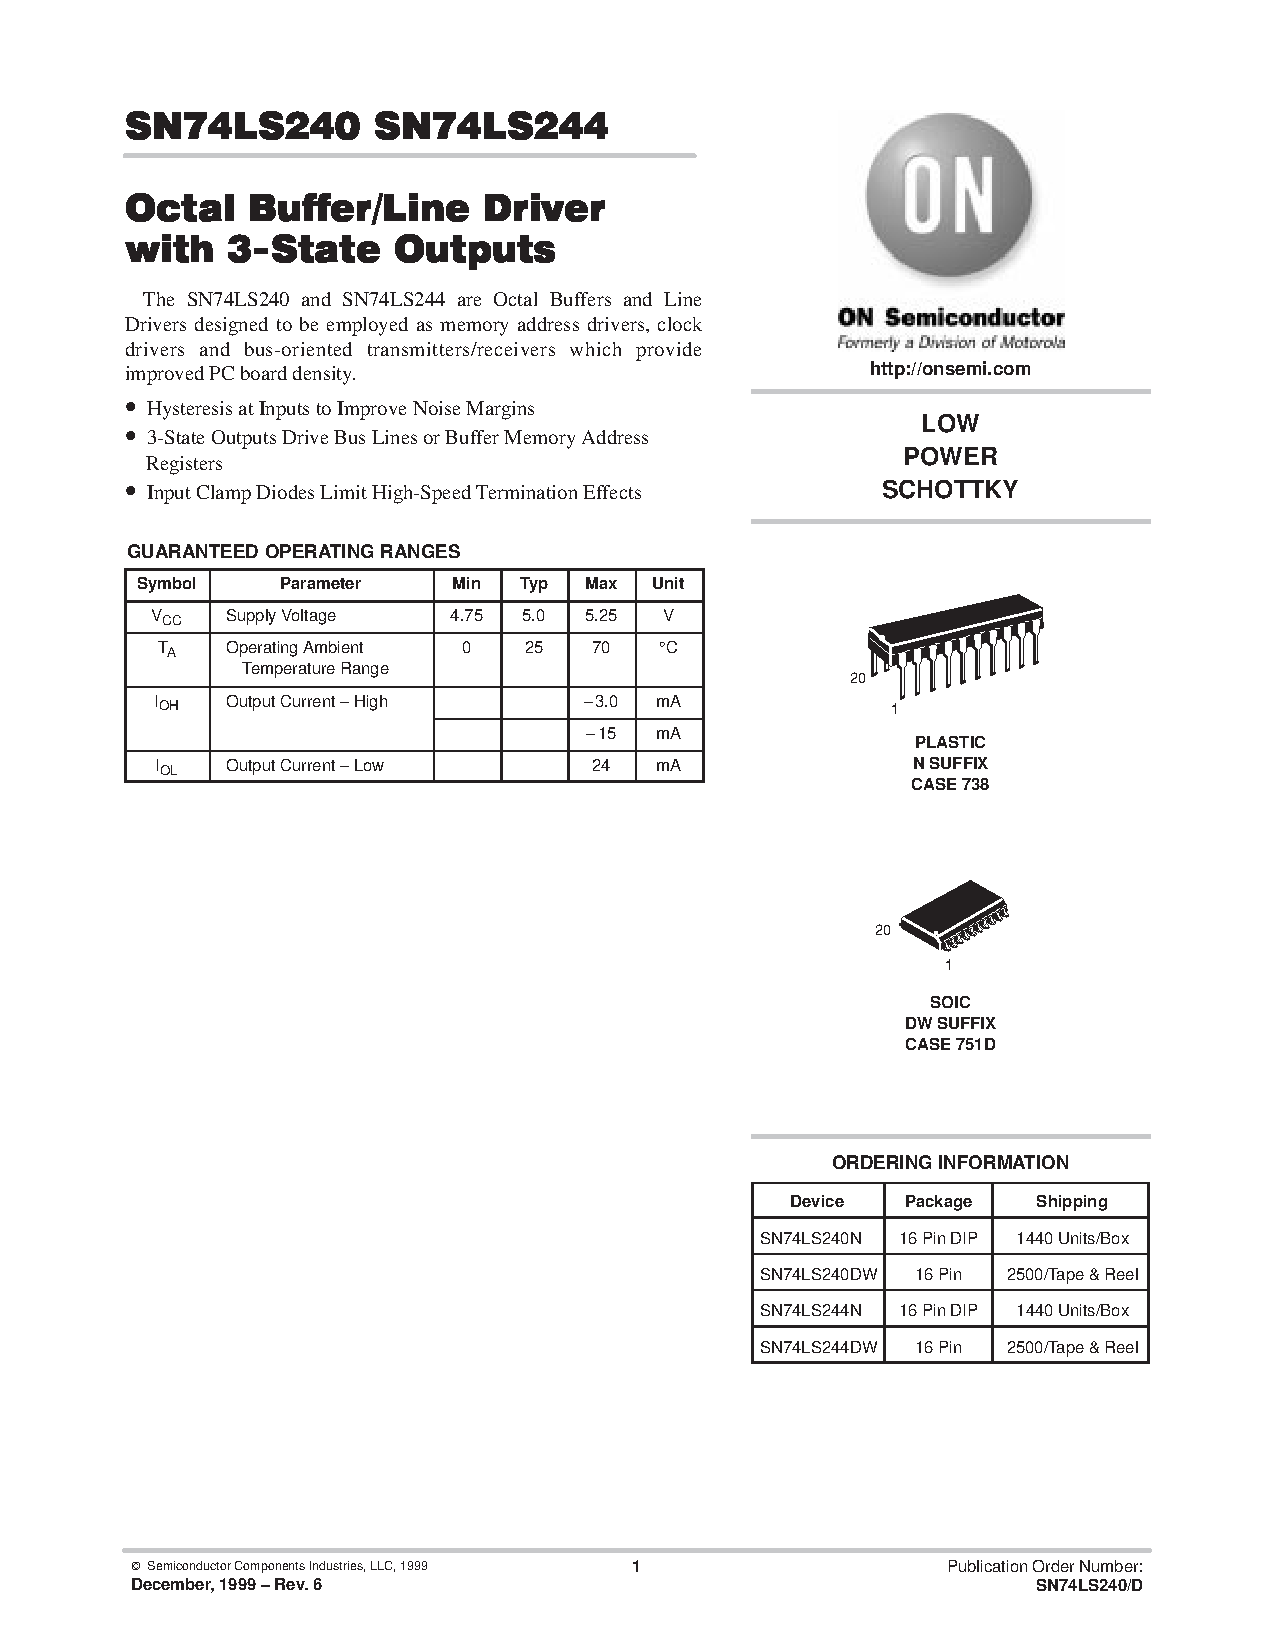
\includepdf[pages=-]{../ref/74LS244.pdf}
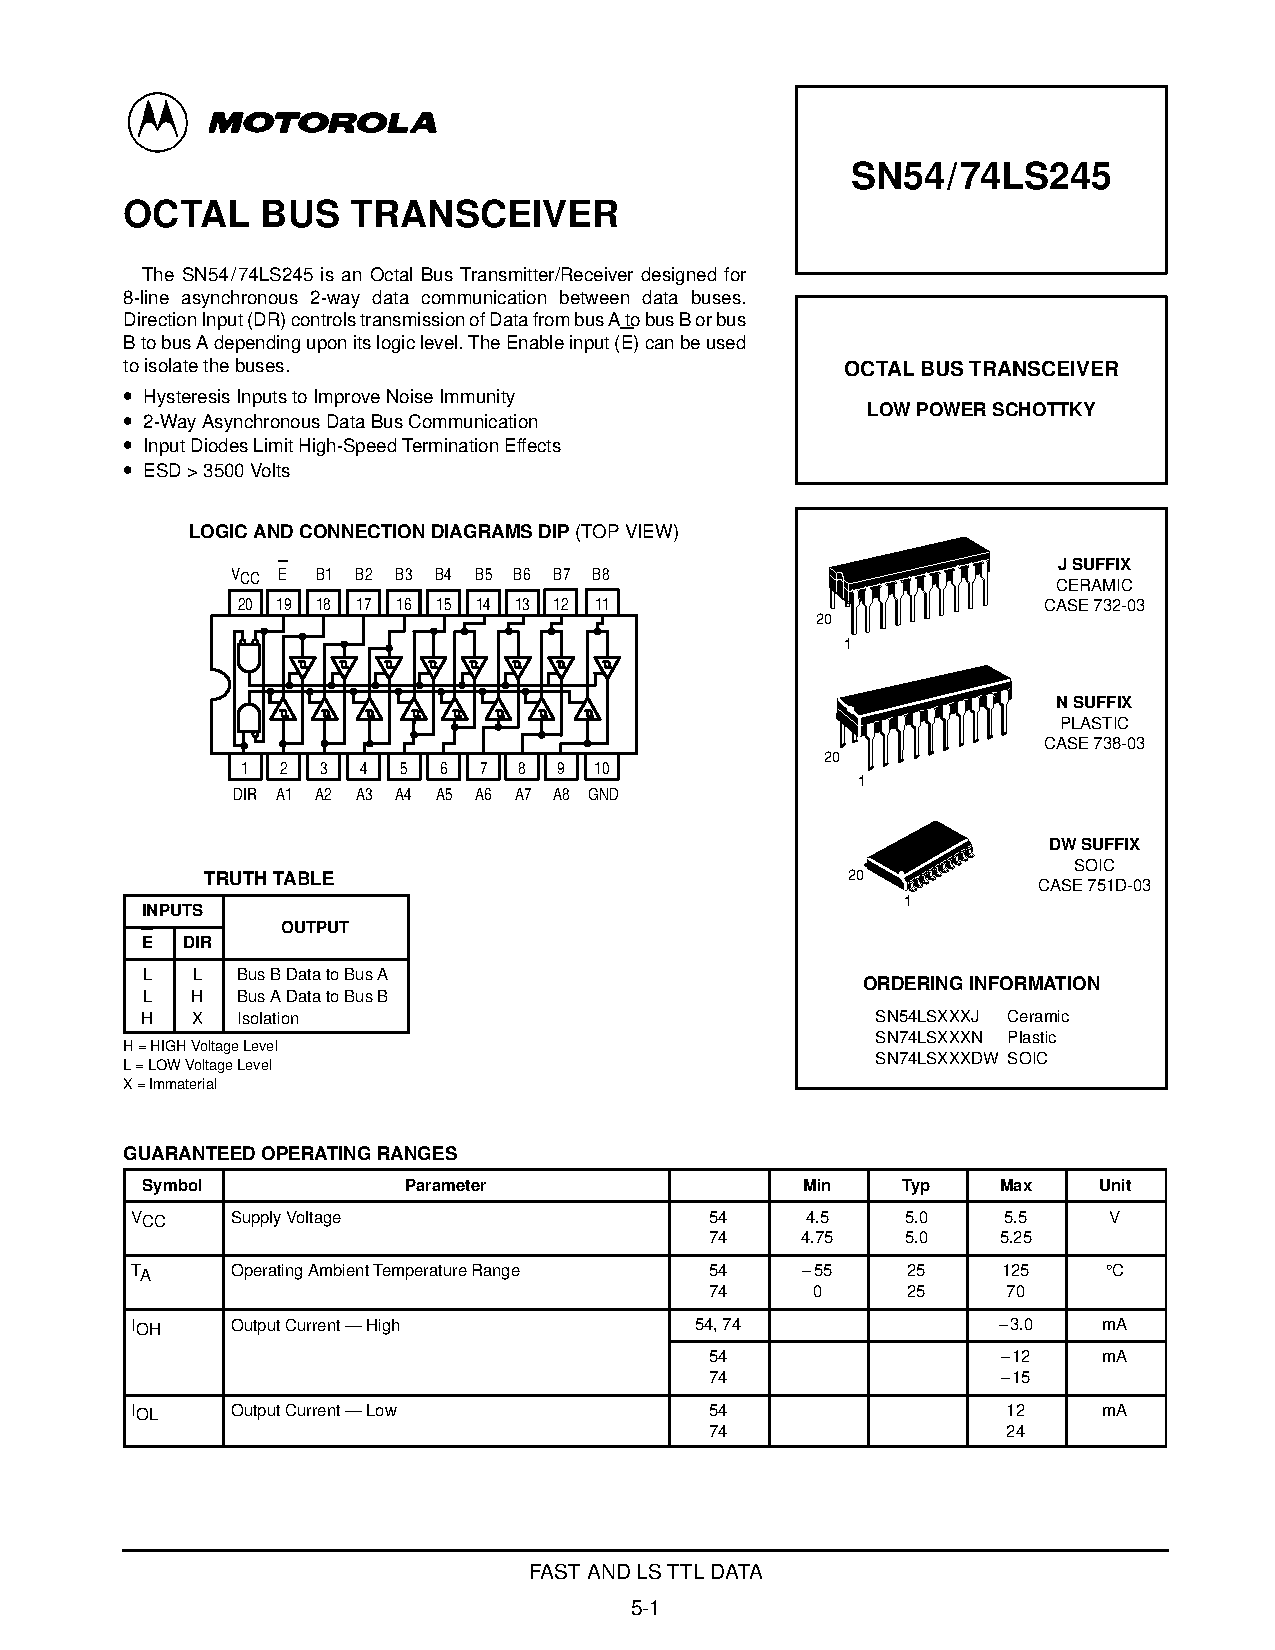
\includepdf[pages=-]{../ref/74LS245.pdf}
% 74*1160 datasheet, part is unused.
%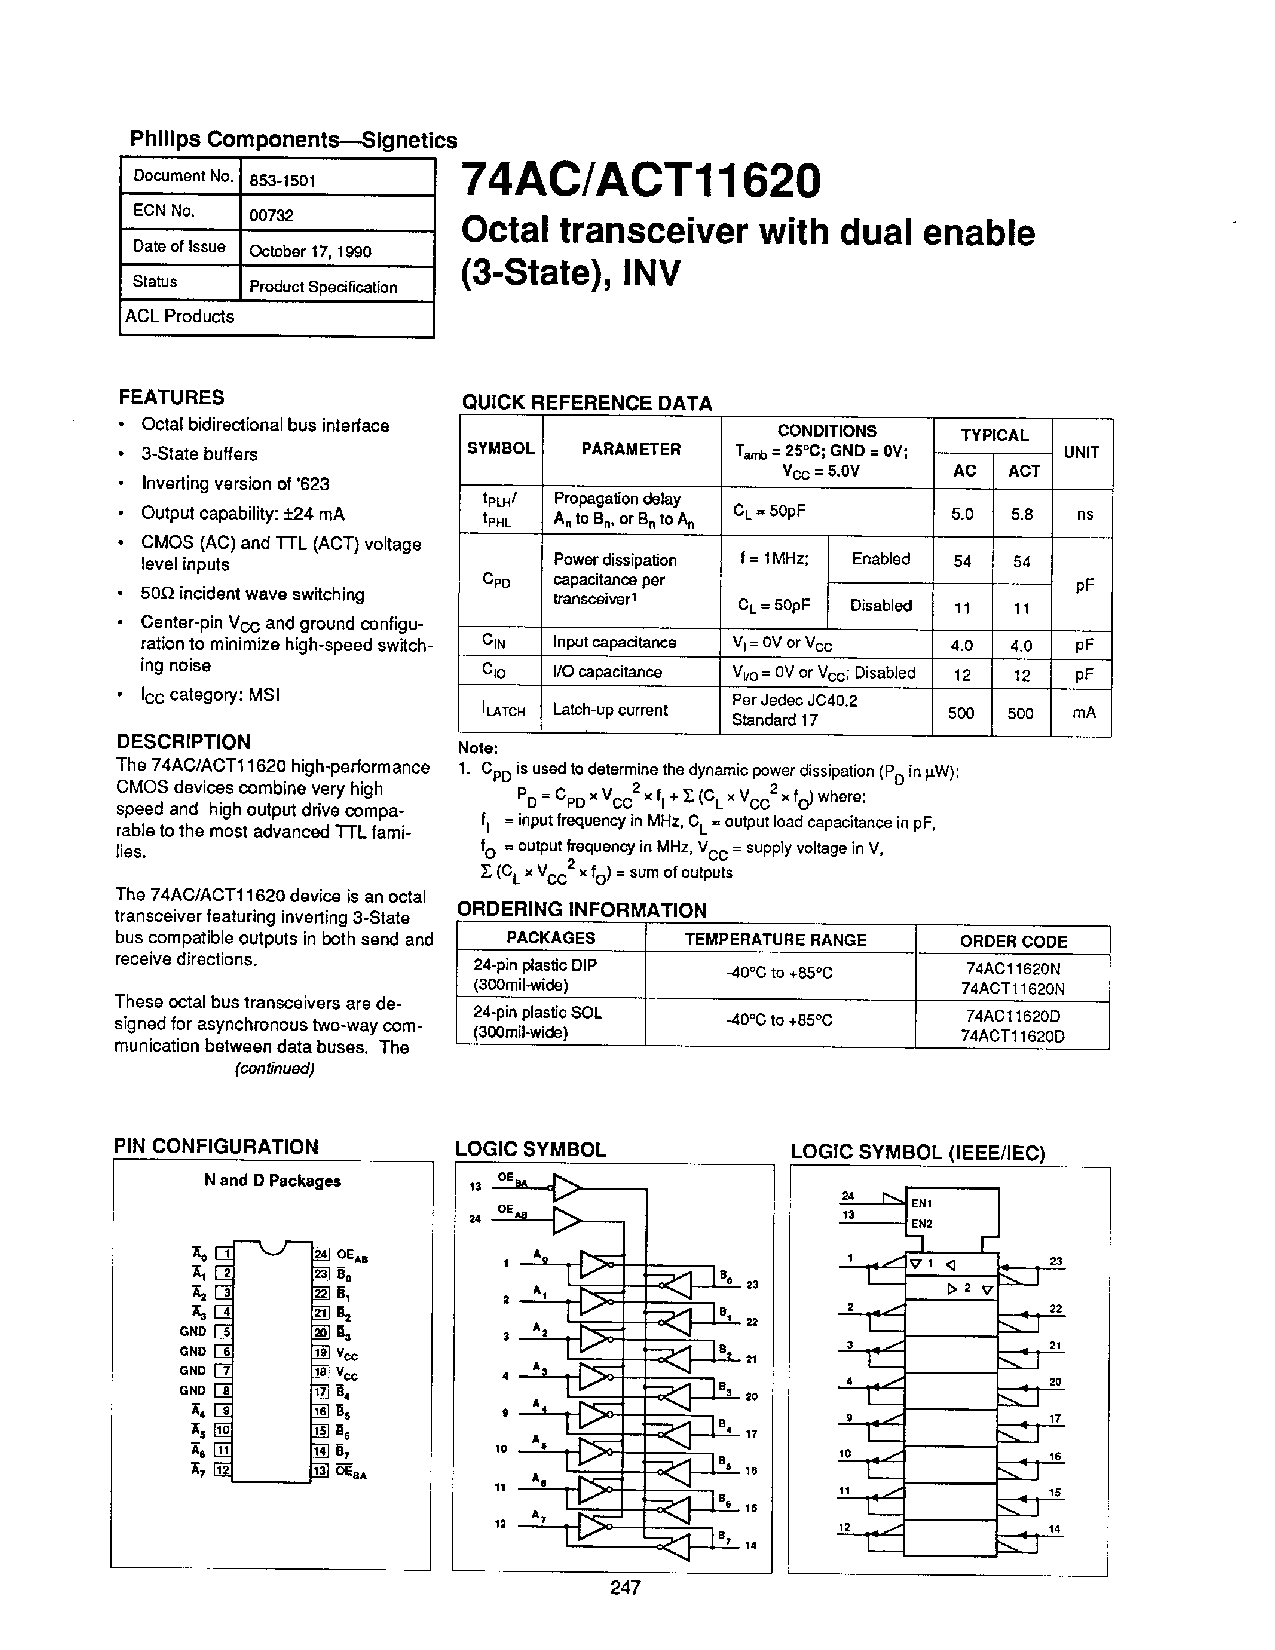
\includepdf[pages=-]{../ref/74AC11620.pdf}

%ADC
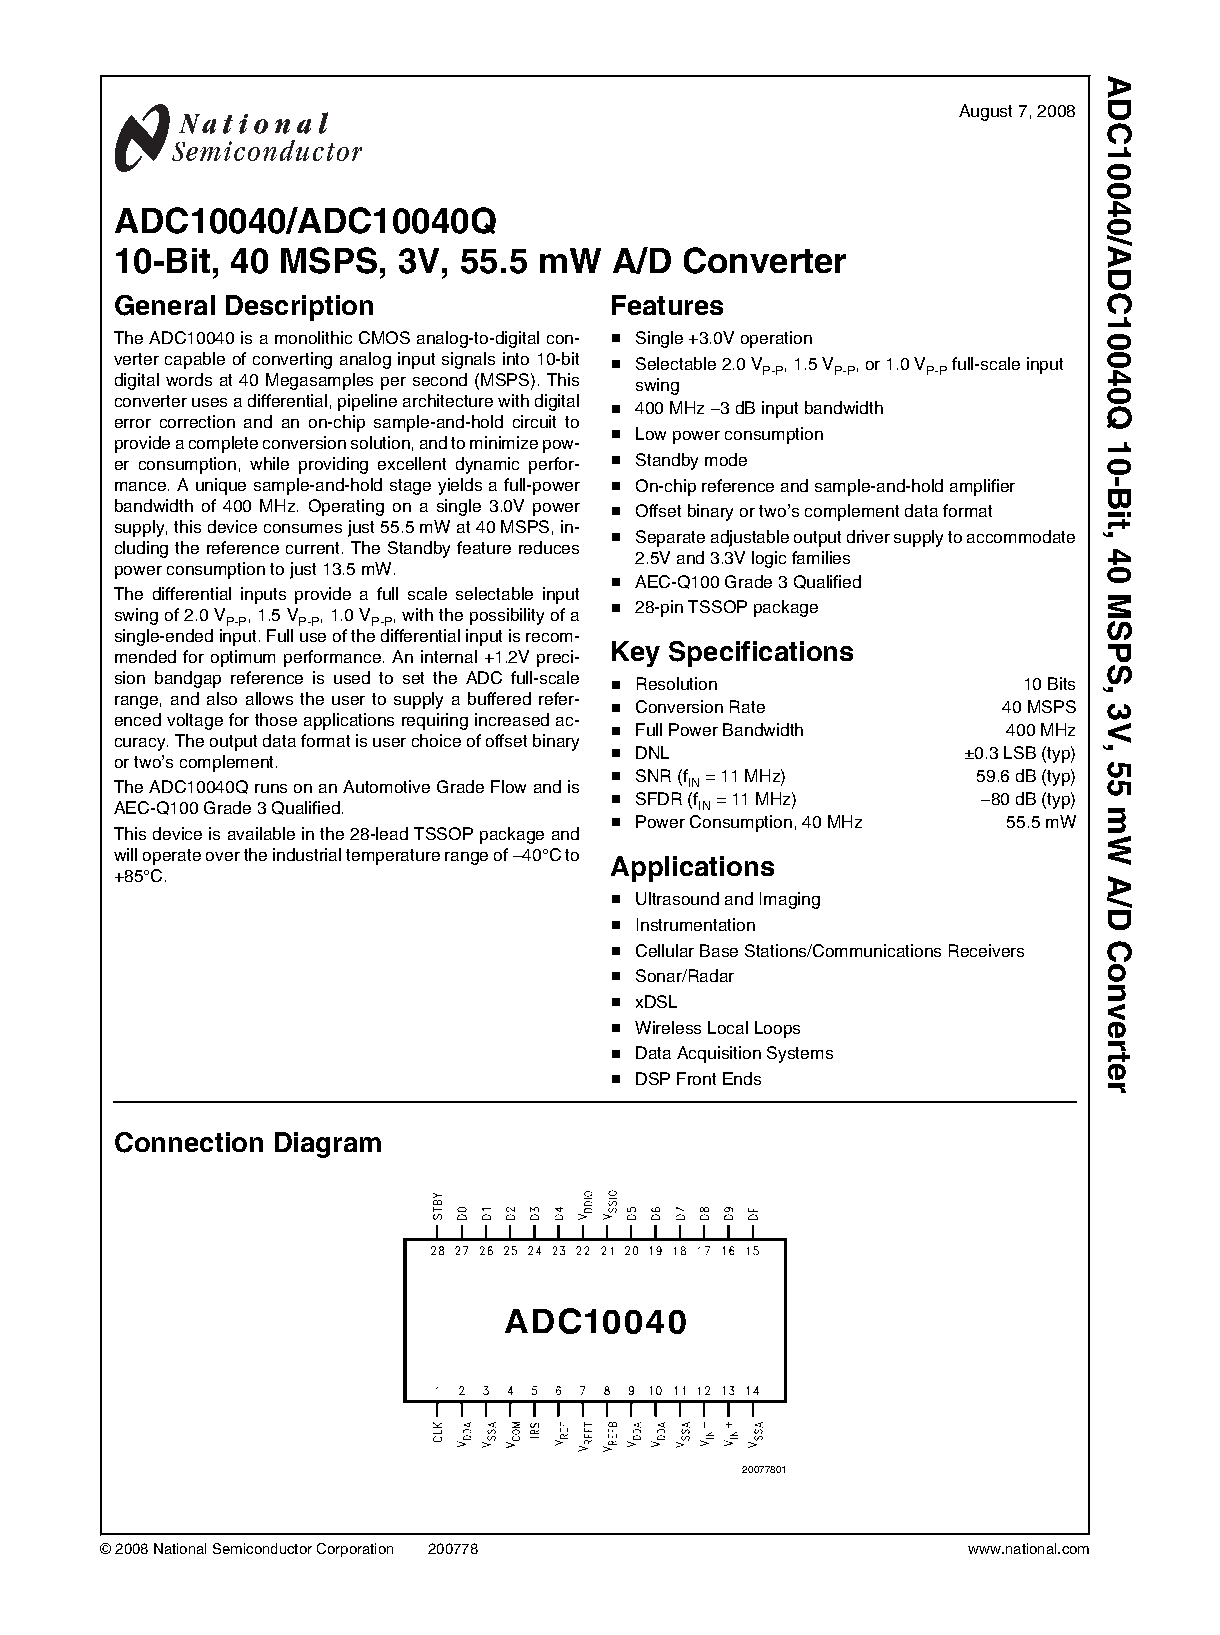
\includepdf[pages=-]{../ref/ADC10040.pdf}

%MAX step-ups
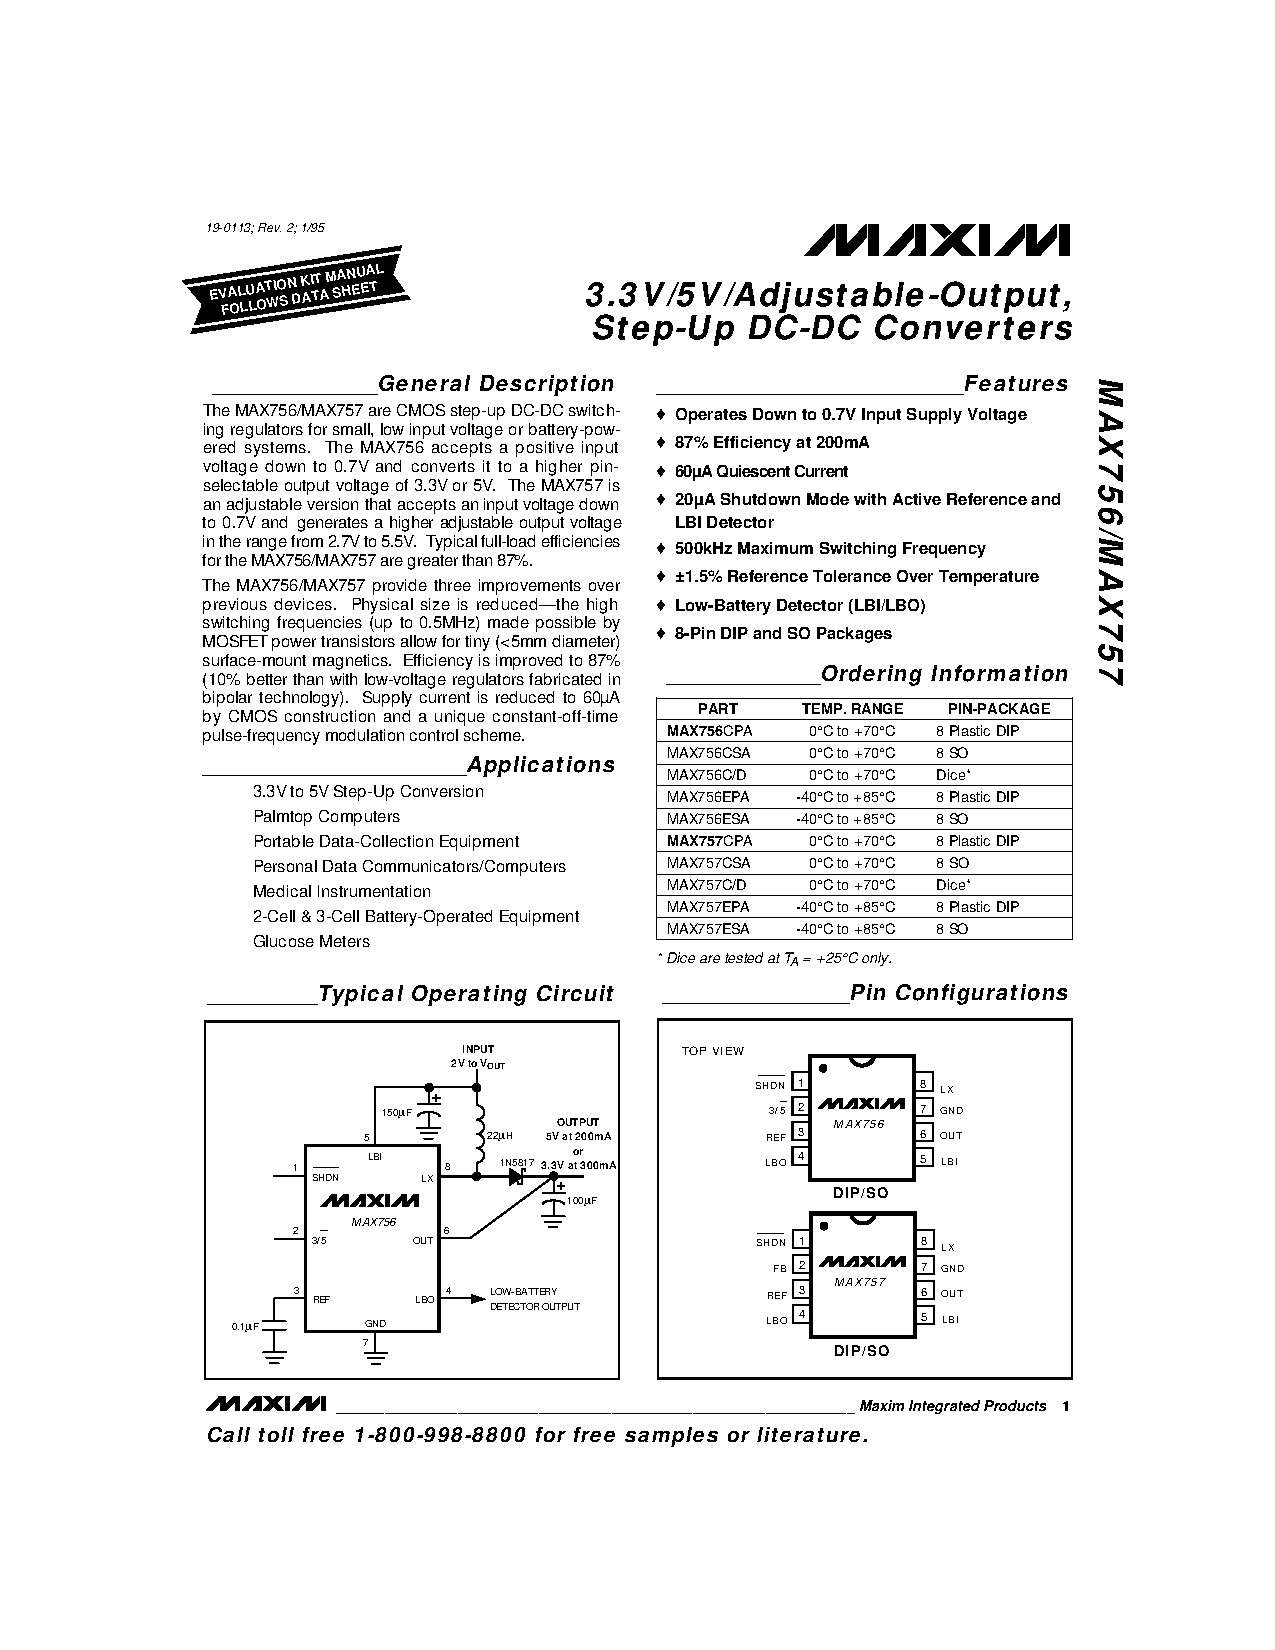
\includepdf[pages=-]{../ref/MAX756-MAX757.pdf}



% All code listings for our project.
\chapter{Software Listings}
%Put all printouts of code listings here.
\lstset{numbers=left, tabsize=2, breakatwhitespace=true}
\lstset{columns=fullflexible}
\lstset{breaklines=true}
\section[Controller Source]{Microcontroller Source Code}

\subsection{Main Control Unit}\index{MCU}\index{Main Control Unit}
\lstset{language=c}
\lstinputlisting[caption=Main Control Unit Header, label=lst:mcu_h]{../src/mcu/main_control.h}
\lstinputlisting[caption=Main Control Unit, label=lst:mcu_c]{../src/mcu/main_control.c}

\subsection{Serial Control Unit}\index{SCU}\index{Serial Control Unit}
\lstinputlisting[caption=Serial Control Unit, label=lst:scu_c]{../src/mcu/usart.c}

\subsection{Common Utilities}
\lstinputlisting[caption=SPI Interface Functions, label=lst:spi_c]{../src/mcu/spi_util.c}
\lstinputlisting[caption=USART Interface Functions, label=lst:usart_c]{../src/mcu/usart_util.c}
\lstinputlisting[caption=Common Defines, label=lst:common_h]{../src/mcu/control_defines.h}

\section{Host PC Software}
\lstset{language=python}
\subsection{Display/Control Interface}
\lstinputlisting[caption=Display/Control Interface, label=lst:inter]{../src/pcsoft/inter.py}

\subsection {Data Acquisition}
\lstinputlisting[caption=Data Acquisition,label=lst:acqdata]{../src/pcsoft/acqdata.py}

\subsection {PC Software Configuration}
\lstinputlisting[caption=Software Configuration, label=lst:pcsoft\_cfg]{../src/pcsoft/pcsoft_cfg.py}

\subsection{Data Display}
\lstset{language=matlab}
\lstinputlisting[caption=Matlab/Octave Data Display,label=lst:dispd]{../src/pcsoft/dispd.m}
\lstinputlisting[caption=Matlab/Octave Get Next File, label=lst:getnextfile]{../src/pcsoft/getnextfile.m}
\lstinputlisting[caption=Matlab/Octave Read/Plot Data, label=lst:readandplot]{../src/pcsoft/readandplot.m}

\end{appendix}
\bibliographystyle{plain}
\bibliography{citations}
\end{document}
